\subsection{Videre arbejde}
Gennem princippet om brugerindragelse valgte vi at skrive et spørgeskema som gav os mulighed for at se om der er nogen relevans for vores forslag. Det lykkedes os også at få kontakt til en enkelt diabetiker som stillede op til interview. Desværre var det ikke muligt at besøge noget sundhedspersonale da Rigshospitalet aldrig vente tilbage på vores henvendelse og Steno først har mulighed for at se os sidst i April.\\
Vores spørgeskemaundersøgelse og interview gav os en generel indikation om at diabetikere benytter mange forskellige sider til mange forskellige opgaver. Størstedelen af vores deltagere har heller ingen kendskab til 'Min Sundhedsplatform'. Dem som benytter siden føler der er meget irrelevant 'spam' og benytter primært siden til at få svar på prøver. Der er bred enighed om at receptfornyelse ville være relevant for siden og være en forbedring af siden, og besvarelserne gør det sandsynligt at denne funktion vil blive benyttet.

\begin{figure}[H]
	\centering
	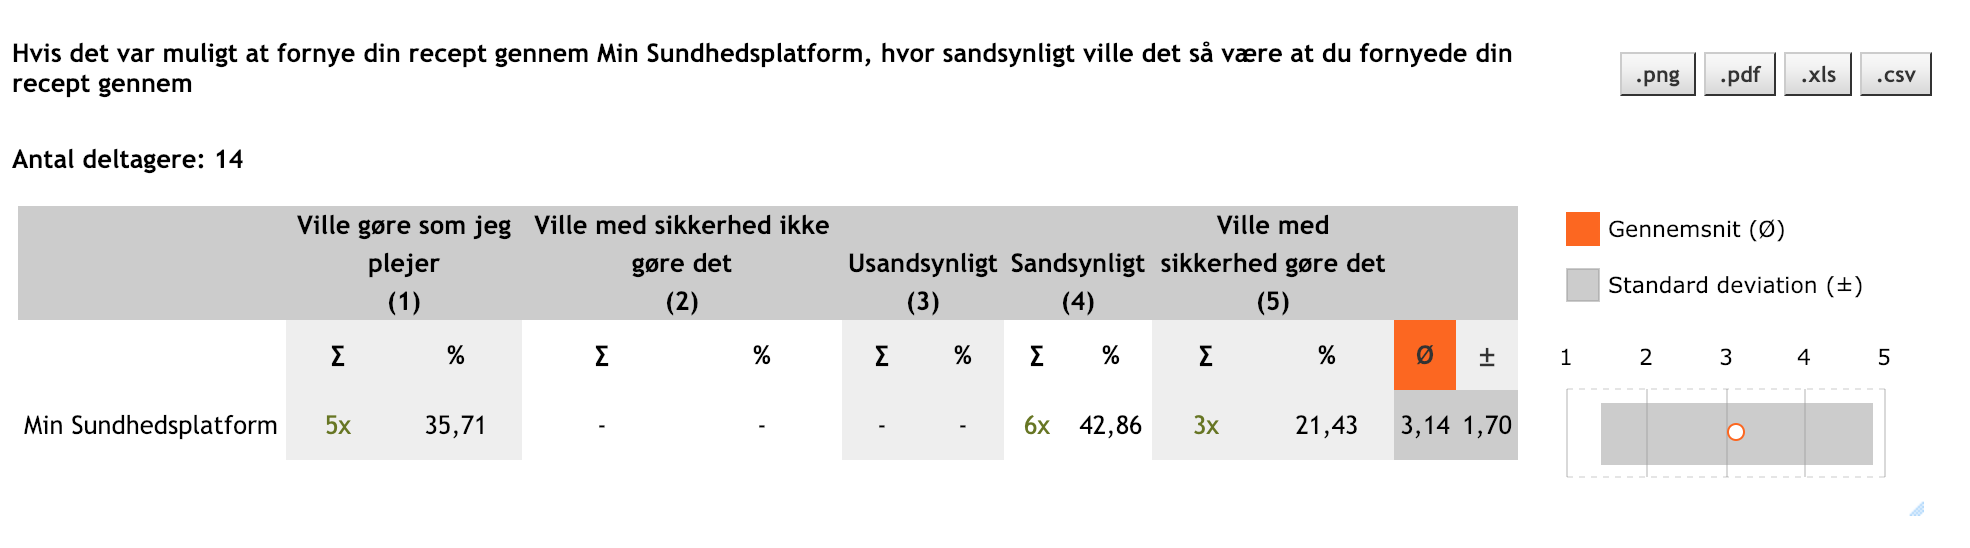
\includegraphics[width=\textwidth]{Materials/Receptfornyelse}
	\caption{Svarfordeling på spørgsmål om receptfornyelse.}
\end{figure}

Undersøgelserne viser at der bliver søgt ny information, men det er lige så tit svaret på spørgsmålet findes på siden som at det ikke gør. Der opbakning om at 'Min Sundhedsplatform' ville være et relevant sted at samle informationen.
 
\begin{figure}[H]
	\centering
	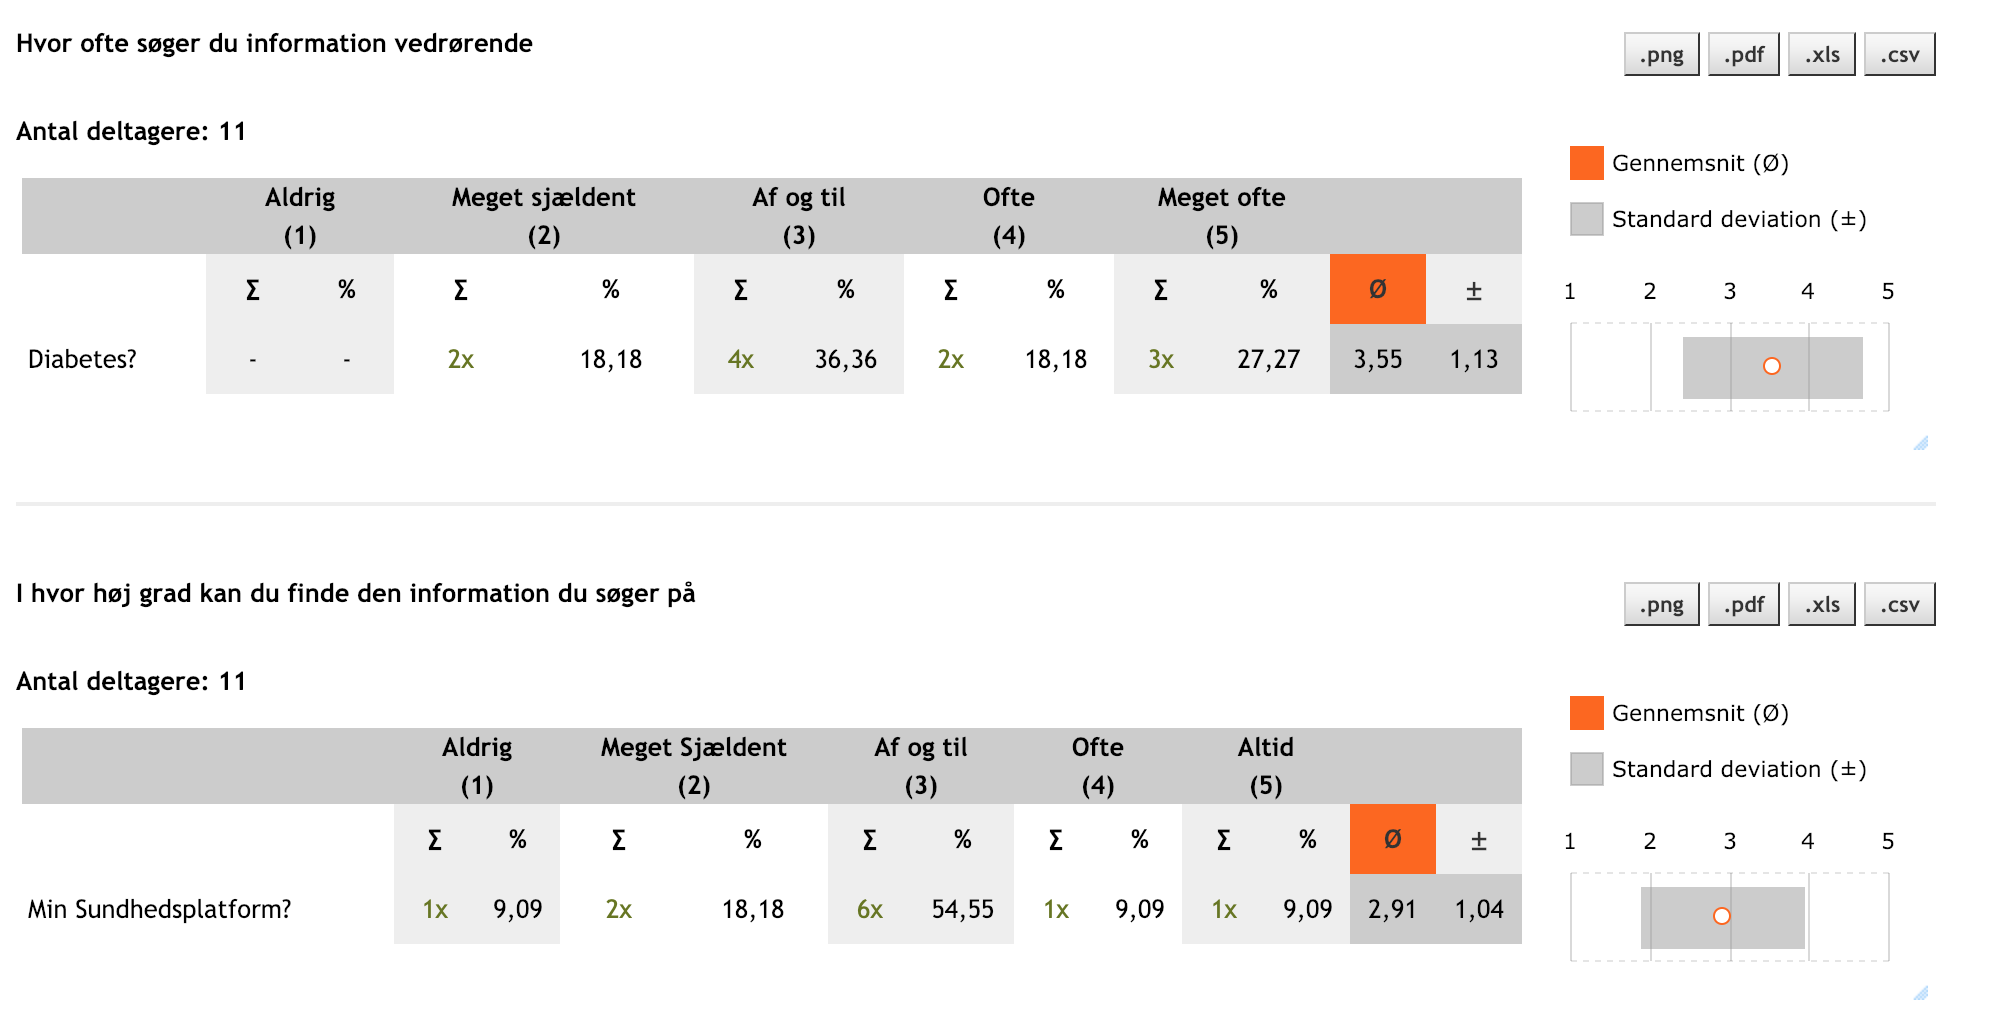
\includegraphics[width=\textwidth]{Materials/SeekingInformation}
	\caption{Svarfordeling på spørgsmål om søgning af information.}
\end{figure}

Der er ikke noget ønske om at møde andre med diabetes gennem siden. Cirka halvdelen af de adspurgte diabetikere deltagere i forskning relateret til diabetes, og der er mange som finder det sandsynligt at deltage i forskning hvis adspurgt. Tilgengæld mener mange det er et 'forkert' sted at tilbyde deltagelse, og finder det mere relevant at blive adspurgt i forbindelse med hospitalsbesøg.\\
Resten af spørgeskemaets resultater kan findes blandt bilagene.\\

Baseret på resultatet af vores interview og spørgeskemaundersøgelse har vi besluttet at projektet vil fokusere på hvordan 'Min Sundhedsplatform' kan blive den eneste side som der er behov for blandt diabetikere. Arbejdet vil involvere samling af funktioner som er spredt på andre sider og at gøre den information som er tilgængelig nem og forståelig for alle.